\clearpage
\section{Multirobot problem}
\subsection{Problem definition and states}

The basic idea is fill the maze with robots, give them instruction simultaneously, while gradually merging them to one point, which is the goal point.

The initial state looks similar to multi robot problem, which is also a 2-D matrix. $k$ equals to number of cell that is not wall.

$$\begin{pmatrix}
x_0 & y_0 \\
x_1 & y_1 \\
\vdots & \vdots \\	
x_{k-1} & y_{k-1}
\end{pmatrix}$$

The key of the problem is to design a consistent heuristic funciton. Which satisfy the formula in previous section. My intuition is approaching the goal while shrinking the range of robot positions. I think calculating the average and standard deviation of all the coordinates is a reasonable approach. The average describe the center of the group, the deviation describes the convergence. 

So, the state of this problem is as following, noted that $[x_i,y_i]$ is a $1\times 2$ matrix :
$$c_{x,y} = \sum^{k-1}_{i=0}[x_i,y_i]/k$$
$$d_{x,y} = ||\sqrt{ c_{x^2,y^2} - (c_{x,y})^2}||$$

Then, the heuristic function would be:
$$h = manhattan(c_{x,y}, g_{x,y}) + d_{x,y}$$

How do I prove that the heuristic function is consistent? First, it apparently satisfy $h(G)=0$, because at that point, all robot will stay at one point, which makes $ d_{x,y} = 0$. Since the point is the goal, which makes, $manhattan(c_{x,y})=0$. As for $h(N) \leq c(N,P)+h(P) $, it is similar to the way that I used to prove monotonic previously. First let's assume an extreme case where there is an empty $N \times N$ maze, and the goal is at the top-right. I do a little math on it, it seems that if $N > 1 or N < -0.4$, the $cost$ is always larger than $h$. It is obvious always satisfied. (Since I must say I am not a mathematician, I'm not sure if I do it right, feel free to discuss with me if you doubt it).

\subsection{Discussions Polynomial-time blind robot planning}
If we take it as k-robot problem, where $k$ equals to number of cell. Then upper bound of the sates should be $(n-w)^k$. However, 

\subsection{Code implementation}

\subsubsection{getSuccessors}

\textbf{Constructors}
I use two different construcors, one is for problem initialization; another is for getting successors during searching. For the first one, basically it just adding robots at every possible position. \textbf{line 14} is a very important methods, and I will talk about that latter.
\begin{lstlisting}[numbers=left]
public BlindRobotNode() {
  allCoord = new HashSet<>();
  cost = 0;
  // initiate the allCoord
  // if it is at start node, where previous = null
  for (int x = 0; x < maze.width; x++) {
    for (int y = 0; y < maze.height; y++) {
      if (maze.getInt(x, y) == 0) {
        Coordinate newNode = new Coordinate(x, y);
        allCoord.add(newNode);
      }
    }
  }
  newCenDev();
}
\end{lstlisting}
The second constructor is also simple, it basically give instructions to robot to move. It there is obstacle, the very robot just stay still.
\begin{lstlisting}[numbers=left]
public BlindRobotNode(Coordinate dxdy, BlindRobotNode prev, double c) {
  // initiate the positions
  allCoord = new HashSet<>();
  cost = c;
  // move all the node in the belief set to direction dxdy
  for (Coordinate xy : prev.allCoord) {
    if (maze.isLegal((int) (xy.x + dxdy.x), (int) (xy.y + dxdy.y))) {
      allCoord.add(new Coordinate(xy.x + dxdy.x, xy.y + dxdy.y));
    } else {
      // if not legal, simply not moving
      allCoord.add(new Coordinate(xy.x, xy.y));
    }
  }
  newCenDev();
}
\end{lstlisting}

\subsubsection{newCenDev}

\textbf{newCenDev} creates the states, calculates the center and the deviation, for all the existing coordinate. Noted that the number of existing coordinate is decreasing, since some robots may merge together.
\begin{lstlisting}[numbers=left]
// dev = E(x^2) - (Ex)^2
private void newCenDev() {
  center = new Coordinate(0, 0);
  sDeviation = new Coordinate(0, 0);
  for (Coordinate xy : allCoord) {
    center.x += xy.x;
    center.y += xy.y;
    sDeviation.x += Math.pow(xy.x, 2);
    sDeviation.y += Math.pow(xy.y, 2);
  }
  center.x /= allCoord.size();
  center.y /= allCoord.size();
  sDeviation.x = Math.pow(sDeviation.x - center.x * center.x, 0.5);
  sDeviation.y = Math.pow(sDeviation.y - center.y * center.y, 0.5);
}
\end{lstlisting}

\subsubsection{Other methods}

\textbf{getSuccessors} turns out to be fairly simple. I just need to move towards 4 directions. 
\begin{lstlisting}[numbers=left]
public ArrayList<SearchNode> getSuccessors() {
  ArrayList<SearchNode> successors = new ArrayList<SearchNode>();
  for (int[] action : actions) {
    Coordinate dxdy = new Coordinate(action[0], action[1]);
    successors.add(new BlindRobotNode(dxdy, this, getCost() + 1.0));
  }
  return successors;
}
\end{lstlisting}

The \textbf{heuristic} method.
\begin{lstlisting}[numbers=left]
@Override
public double heuristic() {
  // manhattan distance metric for simple maze with one agent:
  double dx = coordGoal.x - center.x;
  double dy = coordGoal.y - center.y;
  return Math.abs(dx) + Math.abs(dy) + sDeviation.x + sDeviation.y;
}
\end{lstlisting}











\subsection{Output demonstration}

Output of blind robot in 3x3. (Figure \ref{b-2}):
\begin{lstlisting}[numbers=left]
A*:  
  Nodes explored during search:  15
  Maximum space usage during search 100
  path length: 7
\end{lstlisting}

\begin{figure*}[!t]
\normalsize
\centering
\subfigure[start]{
\label{b-2-0} %% label for first subfigure
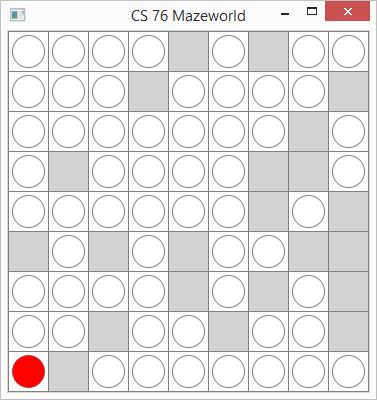
\includegraphics[width=0.206\textwidth]{b-2-1.JPG}}
\subfigure[step 2]{
\label{b-2-0} %% label for first subfigure
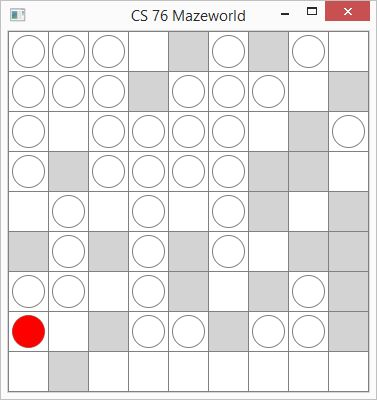
\includegraphics[width=0.206\textwidth]{b-2-2.JPG}}
\subfigure[step 3]{
\label{b-2-0} %% label for first subfigure
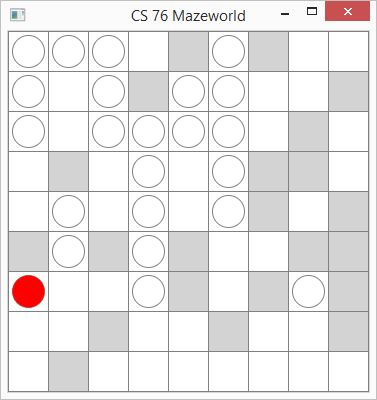
\includegraphics[width=0.206\textwidth]{b-2-3.JPG}}
\subfigure[step 4]{
\label{b-2-0} %% label for first subfigure
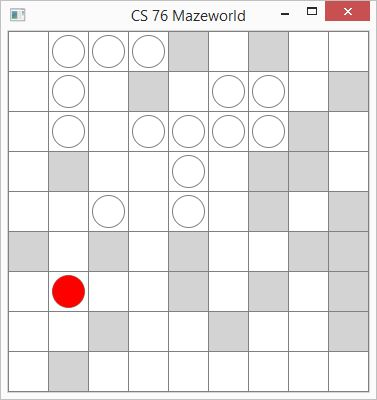
\includegraphics[width=0.206\textwidth]{b-2-4.JPG}}
\subfigure[step 5]{
\label{b-2-0} %% label for first subfigure
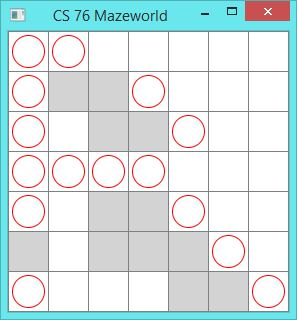
\includegraphics[width=0.206\textwidth]{b-2-5.JPG}}
\subfigure[step 6]{
\label{b-2-0} %% label for first subfigure
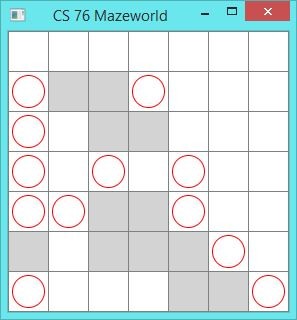
\includegraphics[width=0.206\textwidth]{b-2-6.JPG}}
\subfigure[end]{
\label{b-2-0} %% label for first subfigure
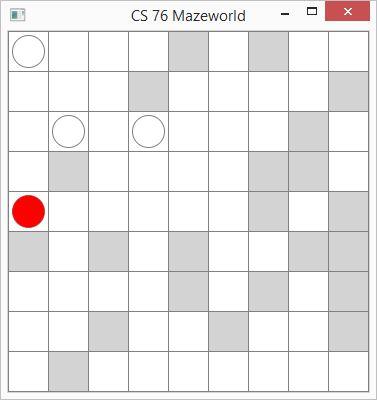
\includegraphics[width=0.206\textwidth]{b-2-7.JPG}}
\caption{Demo of blind robot in 3x3}
\label{b-2} %% label for entire figure
\end{figure*}

\subsection{Output demonstration}

Output of blind robot in 3x3. (Figure \ref{b-2}):
\begin{lstlisting}[numbers=left]
A*:  
  Nodes explored during search:  15
  Maximum space usage during search 100
  path length: 7
\end{lstlisting}

Output of blind robot in 7x7. (Figure \ref{b-2}):
\begin{lstlisting}[numbers=left]
A*:  
  Nodes explored during search:  15
  Maximum space usage during search 100
  path length: 7
\end{lstlisting}

\begin{figure*}[!t]
\normalsize
\centering
\subfigure[start]{
\label{b-1-0} %% label for first subfigure
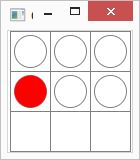
\includegraphics[width=0.206\textwidth]{b-1-2.JPG}}
\subfigure[step 3]{
\label{b-1-0} %% label for first subfigure
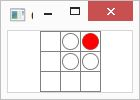
\includegraphics[width=0.206\textwidth]{b-1-3.JPG}}
\subfigure[step 4]{
\label{b-1-0} %% label for first subfigure
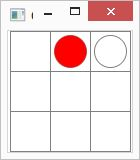
\includegraphics[width=0.206\textwidth]{b-1-4.JPG}}
\subfigure[step 5]{
\label{b-1-0} %% label for first subfigure
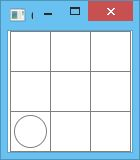
\includegraphics[width=0.206\textwidth]{b-1-5.JPG}}
\subfigure[step 6]{
\label{b-1-0} %% label for first subfigure
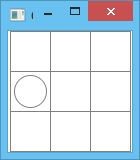
\includegraphics[width=0.206\textwidth]{b-1-6.JPG}}
\subfigure[end]{
\label{b-1-0} %% label for first subfigure
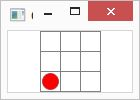
\includegraphics[width=0.206\textwidth]{b-1-7.JPG}}
\caption{Demo of blind robot in 3x3}
\label{b-1} %% label for entire figure
\end{figure*}

\begin{figure*}[!t]
\normalsize
\centering
\subfigure[start]{
\label{b-2-0} %% label for first subfigure
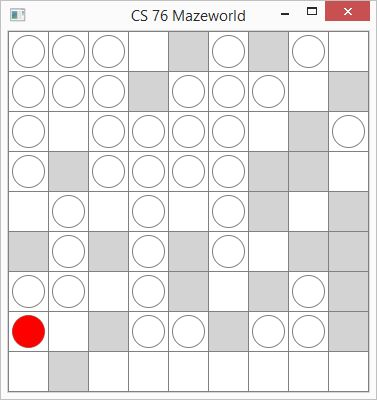
\includegraphics[width=0.206\textwidth]{b-2-2.JPG}}
\subfigure[step 3]{
\label{b-2-0} %% label for first subfigure
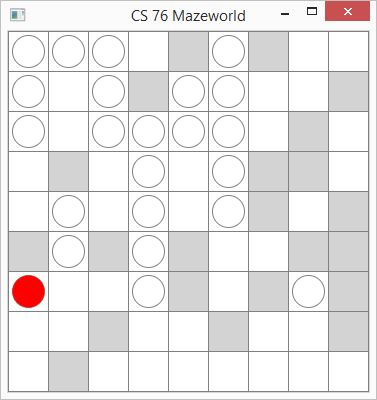
\includegraphics[width=0.206\textwidth]{b-2-3.JPG}}
\subfigure[step 4]{
\label{b-2-0} %% label for first subfigure
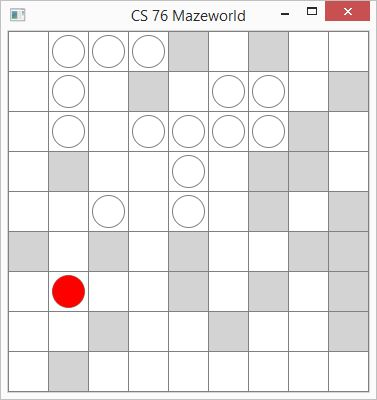
\includegraphics[width=0.206\textwidth]{b-2-4.JPG}}
\subfigure[step 5]{
\label{b-2-0} %% label for first subfigure
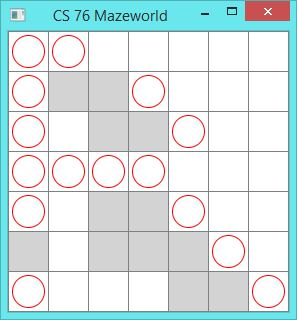
\includegraphics[width=0.206\textwidth]{b-2-5.JPG}}
\subfigure[step 6]{
\label{b-2-0} %% label for first subfigure
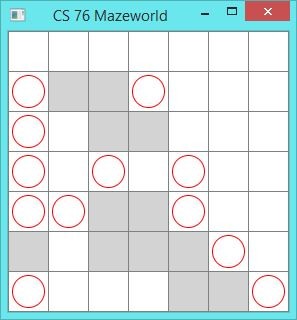
\includegraphics[width=0.206\textwidth]{b-2-6.JPG}}
\subfigure[end]{
\label{b-2-0} %% label for first subfigure
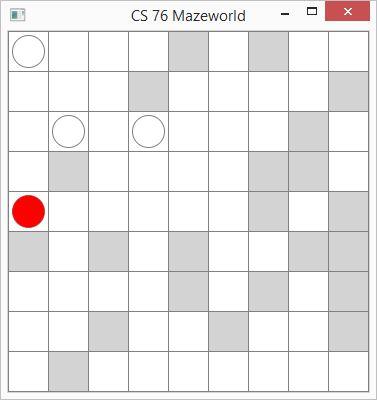
\includegraphics[width=0.206\textwidth]{b-2-7.JPG}}
\caption{Demo of blind robot in 7x7}
\label{b-2} %% label for entire figure
\end{figure*}